\documentclass[xcolor=table]{beamer}
% generated by Madoko, version 1.1.6
%mdk-data-line={1}


\usepackage[heading-base={2},section-num={False},bib-label={hide},fontspec={True}]{madoko2}
%mdk-data-line={1;out\presentation.mdk:79}

    \ifbeamer\relax\else
      \providecommand{\usetheme}[2][]{}
      \providecommand{\usecolortheme}[2][]{}
      \providecommand{\usefonttheme}[2][]{}
      \providecommand{\pause}[1][]{}
      \providecommand{\AtBeginSection}[2][]{}
      \providecommand{\AtBeginSubsection}[2][]{}
      \providecommand{\AtBeginSubsubsection}[2][]{}
      \providecommand{\AtBeginPart}[2][]{}
      \providecommand{\AtBeginLecture}[2][]{}
      \providecommand{\theoremstyle}[2][]{}
      \makeatletter
      \def\newtheorem{\@ifstar\newtheoremx\newtheoremx}
      \makeatother
      \providecommand{\newtheoremx}[3][]{}{}
    \fi
%mdk-data-line={1;out\presentation.mdk:96}

    \ifbeamer\usetheme[]{singapore}\fi
\begin{document}



%mdk-data-line={9}
%mdk-data-line={9}
%mdk-data-line={10}
\mdxtitleblockstart{}
%mdk-data-line={10}
\mdxtitle{{\mdfontsize{3em}\mdline{10}Introduction to Artificial Neural Networks (ANNs)}}%mdk
\mdxauthorstart{\Large{}
%mdk-data-line={15}
\mdxauthorname{{\mdfontsize{1.4em}\mdline{15}Jaya Nilakantan}}%mdk

%mdk-data-line={18}
\mdxauthoraddress{\mdline{18}Dawson College}%mdk

%mdk-data-line={21}
\mdxauthoremail{\mdline{21}jnilakantan@dawsoncollege.qc.ca}%mdk
}\mdxauthorend\mdtitleauthorrunning{}{}\mdxtitleblockend%mdk

%mdk-data-line={12}
\begin{mdframe}%mdk

\frametitle{Recap}\label{heading-sec-recap}%mdk%mdk

%mdk-data-line={13}
\noindent\mdline{13}We\mdline{13}'\mdline{13}ve seen 3 Machine Learning algorithms so far:%mdk

%mdk-data-line={15}
\begin{itemize}%mdk

%mdk-data-line={15}
\item{}
%mdk-data-line={15}
\mdline{15}Linear regression: used to predict a value based on feature(s). Assumes a continuous linear relationship%mdk%mdk

%mdk-data-line={17}
\item{}
%mdk-data-line={17}
\mdline{17}k-nearest neighbours: used to predict a classification based on feature(s).%mdk

%mdk-data-line={18}
\begin{itemize}[noitemsep,topsep=\mdcompacttopsep]%mdk

%mdk-data-line={18}
\item\mdline{18}fine tuning of \mdline{18}$k$\mdline{18} through thew \mdline{18}\emph{k-fold}\mdline{18} cross-validation%mdk
%mdk
\end{itemize}%mdk%mdk

%mdk-data-line={20}
\item{}
%mdk-data-line={20}
\mdline{20}naive Bayes classifier: used to classify based on the assumption that past frequency of features accurately predict the future probability%mdk%mdk
%mdk
\end{itemize}%mdk
%mdk
\end{mdframe}\label{sec-recap}%mdk%mdk

%mdk-data-line={22}
\begin{mdframe}%mdk

\frametitle{What did these algorithms have in common?}\label{heading-sec-what-did-these-algorithms-have-in-common}%mdk%mdk

%mdk-data-line={23}
\begin{itemize}%mdk

%mdk-data-line={23}
\item{}
%mdk-data-line={23}
\mdline{23}supervised learning algorithms: assumes labeled data%mdk%mdk

%mdk-data-line={25}
\item{}
%mdk-data-line={25}
\mdline{25}pretty fast algorithms / optimization algorithms%mdk%mdk

%mdk-data-line={27}
\item{}
%mdk-data-line={27}
\mdline{27}assumes some understanding of the data and the best algorithm%mdk

%mdk-data-line={28}
\begin{itemize}[noitemsep,topsep=\mdcompacttopsep]%mdk

%mdk-data-line={28}
\item\mdline{28}for example, you realize that a linear relationship exists between feature(s) and output%mdk
%mdk
\end{itemize}%mdk%mdk
%mdk
\end{itemize}%mdk
%mdk
\end{mdframe}\label{sec-what-did-these-algorithms-have-in-common}%mdk%mdk

%mdk-data-line={30}
\begin{mdframe}%mdk

\frametitle{So why use neural networks to solve the same type of problems?}\label{heading-sec-so-why-use-neural-networks-to-solve-the-same-type-of-problems}%mdk%mdk

%mdk-data-line={31}
\begin{itemize}%mdk

%mdk-data-line={31}
\item{}
%mdk-data-line={31}
\mdline{31}neural networks can represent almost any function, as stated by the\mdline{31}~\href{https://en.wikipedia.org/wiki/Universal_approximation_theorem}{universal approximation theorem}\mdline{31}.%mdk

%mdk-data-line={32}
\begin{itemize}[noitemsep,topsep=\mdcompacttopsep]%mdk

%mdk-data-line={32}
\item\mdline{32}much much easier than deriving the complicated math for a multi-variate nonlinear relationship%mdk

%mdk-data-line={33}
\item\mdline{33}think about how hard is is to predict the weather%mdk
%mdk
\end{itemize}%mdk%mdk

%mdk-data-line={35}
\item{}
%mdk-data-line={35}
\mdline{35}scale well for huge datasets%mdk%mdk

%mdk-data-line={37}
\item{}
%mdk-data-line={37}
\mdline{37}can yield accuracy that is much better than the statistical/algorithmic machine learning models%mdk%mdk
%mdk
\end{itemize}%mdk
%mdk
\end{mdframe}\label{sec-so-why-use-neural-networks-to-solve-the-same-type-of-problems}%mdk%mdk

%mdk-data-line={41}
\begin{mdframe}%mdk

\frametitle{What are artificial neural networks?}\label{heading-sec-what-are-artificial-neural-networks}%mdk%mdk

%mdk-data-line={43}
\begin{quote}%mdk

%mdk-data-line={43}
\noindent\mdline{43}\dots{}\mdline{43}computing systems vaguely inspired by the biological neural networks that constitute animal brains.\mdline{43}\mdbr
\mdline{44}\textemdash{}\mdline{44}~\href{https://en.wikipedia.org/wiki/Artificial_neural_network}{Wikipedia}\mdline{44}
  \mdline{45} \mdline{45}%mdk
%mdk
\end{quote}%mdk
%mdk
\end{mdframe}\label{sec-what-are-artificial-neural-networks}%mdk%mdk

%mdk-data-line={47}
\begin{mdframe}%mdk

\frametitle{What are artificial neural networks?}\label{heading-sec-what-are-artificial-neural-networks}%mdk%mdk

%mdk-data-line={49}
\noindent\mdline{49} \mdline{49} \mdline{49}%mdk

%mdk-data-line={49}
\begin{quote}%mdk

%mdk-data-line={49}
\noindent\mdline{49}\dots{}\mdline{49}a computing system made up of a number of simple, highly interconnected processing elements, which process information by their dynamic state response to external inputs.\mdline{49}\mdbr
\mdline{50}\textemdash{}\mdline{50}~\href{https://en.wikipedia.org/wiki/Robert_Hecht-Nielsen}{Dr. Robert Hecht-Nielsen}\mdline{50}%mdk
%mdk
\end{quote}%mdk
%mdk
\end{mdframe}\label{sec-what-are-artificial-neural-networks}%mdk%mdk

%mdk-data-line={53}
\begin{mdframe}%mdk

\frametitle{What are artificial neural networks?}\label{heading-sec-what-are-artificial-neural-networks}%mdk%mdk

%mdk-data-line={55}
\begin{quote}%mdk

%mdk-data-line={55}
\noindent\mdline{55}\dots{}\mdline{55}a massively parallel combination of simple processing unit which can acquire knowledge from environment through a learning process and store the knowledge in its connections. \mdline{55}\mdbr
\mdline{56}\textemdash{}\mdline{56}~\href{https://www.eng.mcmaster.ca/ece/people/faculty/simon-haykin}{Simon Haykin}\mdline{56}%mdk
%mdk
\end{quote}%mdk
%mdk
\end{mdframe}\label{sec-what-are-artificial-neural-networks}%mdk%mdk

%mdk-data-line={58}
\begin{mdframe}%mdk

\frametitle{Reasons why neural computation was studied}\label{heading-sec-reasons-why-neural-computation-was-studied}%mdk%mdk

%mdk-data-line={60}
\begin{itemize}[noitemsep,topsep=\mdcompacttopsep]%mdk

%mdk-data-line={60}
\item\mdline{60}to understand how the brain works

%mdk-data-line={61}
\begin{itemize}[noitemsep,topsep=\mdcompacttopsep]%mdk

%mdk-data-line={61}
\item\mdline{61}computer simulation won\mdline{61}'\mdline{61}t harm someone!%mdk
%mdk
\end{itemize}%mdk%mdk

%mdk-data-line={63}
\item\mdline{63}to implement the same kind of parallel computation that neurons perform

%mdk-data-line={64}
\begin{itemize}[noitemsep,topsep=\mdcompacttopsep]%mdk

%mdk-data-line={64}
\item\mdline{64}very different from out typical sequential algorithms%mdk

%mdk-data-line={65}
\item\mdline{65}should be good at things the brain is good at (e.g., vision, recognition)%mdk

%mdk-data-line={66}
\item\mdline{66}should be bad at thing the brain is bad at (e.g., computation like 23 x 71)%mdk
%mdk
\end{itemize}%mdk%mdk

%mdk-data-line={68}
\item\mdline{68}to solve problems using algorithms \mdline{68}\emph{inspired}\mdline{68} by how the brain works

%mdk-data-line={69}
\begin{itemize}[noitemsep,topsep=\mdcompacttopsep]%mdk

%mdk-data-line={69}
\item\mdline{69}but not necessarily exactly how the brain would do it%mdk
%mdk
\end{itemize}%mdk%mdk
%mdk
\end{itemize}%mdk
%mdk
\end{mdframe}\label{sec-reasons-why-neural-computation-was-studied}%mdk%mdk

%mdk-data-line={71}
\begin{mdframe}%mdk

\frametitle{Biological motivation}\label{heading-sec-biological-motivation}%mdk%mdk

%mdk-data-line={73}
\begin{itemize}%mdk

%mdk-data-line={73}
\item{}
%mdk-data-line={73}
\mdline{73}the basic computational unit of the human brain is a \mdline{73}\emph{neuron}\mdline{73}%mdk%mdk

%mdk-data-line={75}
\item{}
%mdk-data-line={75}
\mdline{75}the human brain is composed of \mdline{75}\textasciitilde{}\mdline{75}10\mdline{75}\mdsup{11}\mdline{75} neurons%mdk%mdk

%mdk-data-line={77}
\item{}
%mdk-data-line={77}
\mdline{77}they connect to each other through  \mdline{77}\emph{synapses}\mdline{77}%mdk%mdk

%mdk-data-line={79}
\item{}
%mdk-data-line={79}
\mdline{79}each connection is \mdline{79}\emph{weighted}\mdline{79} according to its importance%mdk%mdk
%mdk
\end{itemize}%mdk
%mdk
\end{mdframe}\label{sec-biological-motivation}%mdk%mdk

%mdk-data-line={81}
\begin{mdframe}%mdk

\frametitle{Biological neuron}\label{heading-sec-biological-neuron}%mdk%mdk

%mdk-data-line={83}
\noindent\mdline{83}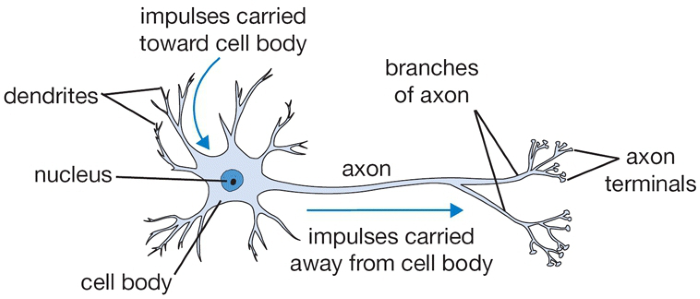
\includegraphics[keepaspectratio=true,width=\dimmin{}{\dimwidth{0.90}}]{images/neuron}{}\mdline{83}%mdk

%mdk-data-line={87}
\begin{itemize}%mdk

%mdk-data-line={87}
\item{}
%mdk-data-line={87}
\mdline{87}signals from axons of previous neurons to dendrites%mdk%mdk

%mdk-data-line={89}
\item{}
%mdk-data-line={89}
\mdline{89}spike of activity in the axon\mdline{89} \mdline{89}-\mdline{89}\textgreater{}\mdline{89} charge through the synapse into the next neuron%mdk%mdk

%mdk-data-line={91}
\item{}
%mdk-data-line={91}
\mdline{91}generates the spike if enough charges have flowed through its dendrites%mdk%mdk

%mdk-data-line={93}
\item{}
%mdk-data-line={93}
\mdline{93}synapses adapt =\mdline{93}\textgreater{}\mdline{93} this is learning%mdk%mdk
%mdk
\end{itemize}%mdk
%mdk
\end{mdframe}\label{sec-biological-neuron}%mdk%mdk

%mdk-data-line={95}
\begin{mdframe}%mdk

\frametitle{How the brain works (\href{http://www.cs.toronto.edu/~hinton/}{Hinton}'s abridged version)}\label{heading-sec-how-the-brain-works-hintonhttp-wwwcstorontoeduhintons-abridged-version}%mdk%mdk

%mdk-data-line={97}
\begin{itemize}%mdk

%mdk-data-line={97}
\item{}
%mdk-data-line={97}
\mdline{97}each neuron receives inputs from 1 or more other neurons%mdk%mdk

%mdk-data-line={99}
\item{}
%mdk-data-line={99}
\mdline{99}the effect of each input on the neuron is controlled by a synaptic weight%mdk

%mdk-data-line={100}
\begin{itemize}[noitemsep,topsep=\mdcompacttopsep]%mdk

%mdk-data-line={100}
\item\mdline{100}positive or negative%mdk
%mdk
\end{itemize}%mdk%mdk

%mdk-data-line={102}
\item{}
%mdk-data-line={102}
\mdline{102}the synaptic weight adapts\mdline{102} \mdline{102}-\mdline{102}\textgreater{}\mdline{102} this is learning%mdk%mdk
%mdk
\end{itemize}%mdk
%mdk
\end{mdframe}\label{sec-how-the-brain-works-hintonhttp-wwwcstorontoeduhintons-abridged-version}%mdk%mdk

%mdk-data-line={104}
\begin{mdframe}%mdk

\frametitle{Artificial neuron - example: Linear neuron}\label{heading-sec-artificial-neuron---example--linear-neuron}%mdk%mdk

%mdk-data-line={106}
\noindent\mdline{106}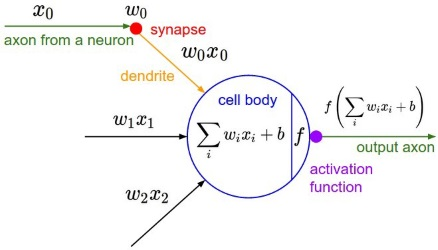
\includegraphics[keepaspectratio=true,width=\dimmin{}{\dimwidth{0.90}}]{images/artneuron}{}\mdline{106}%mdk

%mdk-data-line={110}
\begin{itemize}%mdk

%mdk-data-line={110}
\item{}
%mdk-data-line={110}
\mdline{110}each input has a weight: the relative importance of that input vs the other%mdk%mdk

%mdk-data-line={112}
\item{}
%mdk-data-line={112}
\mdline{112}sum of all the weighted inputs\mdline{112} \mdline{112}+ bias\mdline{112} \mdline{112}-\mdline{112}\textgreater{}\mdline{112} activation function\mdline{112} \mdline{112}-\mdline{112}\textgreater{}\mdline{112} output through the axon to the next neurons%mdk%mdk
%mdk
\end{itemize}%mdk
%mdk
\end{mdframe}\label{sec-artificial-neuron---example--linear-neuron}%mdk%mdk

%mdk-data-line={114}
\begin{mdframe}%mdk

\frametitle{Artificial neuron - example: Binary threshold neuron}\label{heading-sec-artificial-neuron---example--binary-threshold-neuron}%mdk%mdk

%mdk-data-line={116}
\begin{itemize}%mdk

%mdk-data-line={116}
\item{}
%mdk-data-line={116}
\mdline{116}sum of all the weighted inputs\mdline{116} \mdline{116}+ bias%mdk%mdk

%mdk-data-line={118}
\item{}
%mdk-data-line={118}
\mdline{118}if it exceeds a threshold=\mdline{118}\textgreater{}\mdline{118} output of 1, else output of 0%mdk%mdk

%mdk-data-line={120}
\item{}
%mdk-data-line={120}
\mdline{120}think of it as logical combination of True and False signals%mdk%mdk
%mdk
\end{itemize}%mdk
%mdk
\end{mdframe}\label{sec-artificial-neuron---example--binary-threshold-neuron}%mdk%mdk

%mdk-data-line={122}
\begin{mdframe}%mdk

\frametitle{General idea behind ANNs}\label{heading-sec-general-idea-behind-anns}%mdk%mdk

%mdk-data-line={124}
\begin{itemize}%mdk

%mdk-data-line={124}
\item{}
%mdk-data-line={124}
\mdline{124}the weights \mdline{124}\emph{w}\mdline{124} are learnable%mdk%mdk

%mdk-data-line={126}
\item{}
%mdk-data-line={126}
\mdline{126}they control the strength of the influence of one neuron on another%mdk%mdk

%mdk-data-line={128}
\item{}
%mdk-data-line={128}
\mdline{128}weights can be positive (\mdline{128}\textquotedblleft{}excite\textquotedblright{}\mdline{128} the next neuron, causing the sum to exceed the theshold so it fires) or negative (\mdline{128}\textquotedblleft{}inhibit\textquotedblright{}\mdline{128} the next neuron from firing)%mdk%mdk

%mdk-data-line={130}
\item{}
%mdk-data-line={130}
\mdline{130}activation function models the firing rate\mdline{130} \mdline{130}- frequency of spikes on the axon%mdk%mdk
%mdk
\end{itemize}%mdk
%mdk
\end{mdframe}\label{sec-general-idea-behind-anns}%mdk%mdk

%mdk-data-line={132}
\begin{mdframe}%mdk

\frametitle{ANN architecture - Feedforward}\label{heading-sec-ann-architecture---feedforward}%mdk%mdk

%mdk-data-line={134}
\begin{itemize}[noitemsep,topsep=\mdcompacttopsep]%mdk

%mdk-data-line={134}
\item\mdline{134}Feedforward neurons only send information in one direction: the connections can never form a circle%mdk
%mdk
\end{itemize}%mdk
%mdk
\end{mdframe}\label{sec-ann-architecture---feedforward}%mdk%mdk

%mdk-data-line={136}
\begin{mdframe}%mdk

\frametitle{Single layer Perceptron}\label{heading-sec-single-layer-perceptron}%mdk%mdk

%mdk-data-line={138}
\noindent\mdline{138}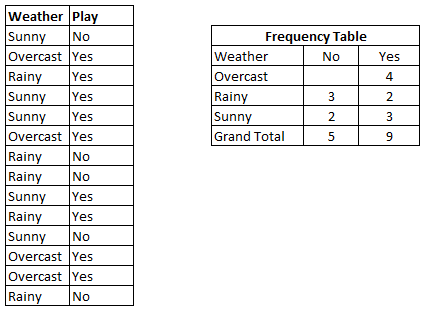
\includegraphics[keepaspectratio=true,width=\dimmin{}{\dimwidth{0.90}}]{images/Capture}{}\mdline{138}%mdk

%mdk-data-line={143}
\begin{itemize}%mdk

%mdk-data-line={143}
\item{}
%mdk-data-line={143}
\mdline{143}simplest feedforward ANN%mdk%mdk

%mdk-data-line={145}
\item{}
%mdk-data-line={145}
\mdline{145}input (training/test data) feeds the output layer based on weights%mdk%mdk

%mdk-data-line={147}
\item{}
%mdk-data-line={147}
\mdline{147}no computations done at input, so it is not counted as a layer%mdk%mdk
%mdk
\end{itemize}%mdk
%mdk
\end{mdframe}\label{sec-single-layer-perceptron}%mdk%mdk

%mdk-data-line={149}
\begin{mdframe}%mdk

\frametitle{A very simple example (source: Hinton)}\label{heading-sec-a-very-simple-example-source--hinton}%mdk%mdk

%mdk-data-line={151}
\noindent\mdline{151}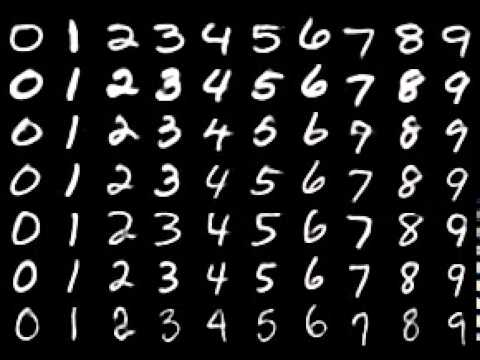
\includegraphics[keepaspectratio=true,width=\dimmin{}{\dimwidth{0.90}}]{images/mnist}{}\mdline{151}%mdk

%mdk-data-line={155}
\noindent\mdline{155}Consider the famous MNIST database of handwritten digits. It is often used for classification experiments.%mdk
%mdk
\end{mdframe}\label{sec-a-very-simple-example-source--hinton}%mdk%mdk

%mdk-data-line={157}
\begin{mdframe}%mdk

\frametitle{Solving with a Single layer perceptron}\label{heading-sec-solving-with-a-single-layer-perceptron}%mdk%mdk

%mdk-data-line={159}
\begin{itemize}[noitemsep,topsep=\mdcompacttopsep]%mdk

%mdk-data-line={159}
\item{}
%mdk-data-line={159}
\mdline{159}each digit is 28x28 bitmap\mdline{159} \mdline{159}-\mdline{159}\textgreater{}\mdline{159} consider that there are 784 inputs, one for each pixel%mdk%mdk

%mdk-data-line={161}
\item{}
%mdk-data-line={161}
\mdline{161}input value represents the pixel intensity%mdk%mdk

%mdk-data-line={163}
\item\mdline{163}the weight of each pixel is initially randomly chosen

%mdk-data-line={164}
\begin{itemize}[noitemsep,topsep=\mdcompacttopsep]%mdk

%mdk-data-line={164}
\item\mdline{164}the weights represent the \mdline{164}\textquotedblleft{}votes\textquotedblright{}\mdline{164} that each pixel has regarding the output(s)%mdk

%mdk-data-line={165}
\item\mdline{165}each pixel can vote for several different outputs%mdk
%mdk
\end{itemize}%mdk%mdk

%mdk-data-line={167}
\item\mdline{167}the output layer are the 9 possible digits. In other words, the possible classifications.

%mdk-data-line={168}
\begin{itemize}[noitemsep,topsep=\mdcompacttopsep]%mdk

%mdk-data-line={168}
\item\mdline{168}the shape with the most votes wins%mdk
%mdk
\end{itemize}%mdk%mdk
%mdk
\end{itemize}%mdk
%mdk
\end{mdframe}\label{sec-solving-with-a-single-layer-perceptron}%mdk%mdk

%mdk-data-line={170}
\begin{mdframe}%mdk

\frametitle{How does the learning happen?}\label{heading-sec-how-does-the-learning-happen}%mdk%mdk

%mdk-data-line={172}
\begin{itemize}%mdk

%mdk-data-line={172}
\item{}
%mdk-data-line={172}
\mdline{172}after every training sample, check the guess with the actual shape%mdk%mdk

%mdk-data-line={174}
\item{}
%mdk-data-line={174}
\mdline{174}for every correct guess, increment the weights from the active pixels to the correct class%mdk%mdk

%mdk-data-line={176}
\item{}
%mdk-data-line={176}
\mdline{176}decrement the weights from the active pixels to any wrong guess%mdk%mdk
%mdk
\end{itemize}%mdk
%mdk
\end{mdframe}\label{sec-how-does-the-learning-happen}%mdk%mdk

%mdk-data-line={178}
\begin{mdframe}%mdk

\frametitle{Results (simple PHP code)}\label{heading-sec-results-simple-php-code}%mdk%mdk

%mdk-data-line={179}
\noindent\mdline{179}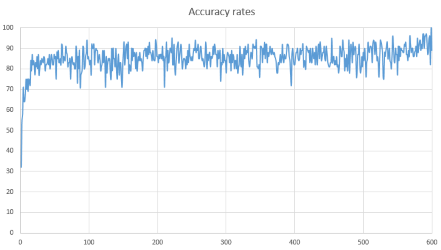
\includegraphics[keepaspectratio=true,width=\dimmin{}{\dimwidth{0.90}}]{images/php1layer}{}\mdline{179}%mdk

%mdk-data-line={184}
\begin{itemize}%mdk

%mdk-data-line={184}
\item{}
%mdk-data-line={184}
\mdline{184}a one-layer network is equivalent to a template for each shap: the winner is the template with that highest overlap%mdk%mdk

%mdk-data-line={186}
\item{}
%mdk-data-line={186}
\mdline{186}hand-written shapes have too much variance: there will always be a relatively high error rate with this approach%mdk%mdk
%mdk
\end{itemize}%mdk
%mdk
\end{mdframe}\label{sec-results-simple-php-code}%mdk%mdk

%mdk-data-line={188}
\begin{mdframe}%mdk

\frametitle{Multi-layer perceptron}\label{heading-sec-multi-layer-perceptron}%mdk%mdk

%mdk-data-line={189}
\noindent\mdline{189}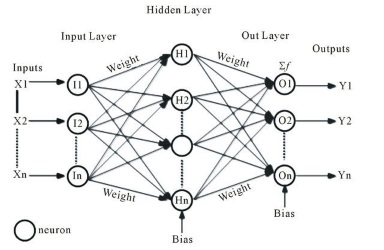
\includegraphics[keepaspectratio=true,width=\dimmin{}{\dimwidth{0.90}}]{images/multiperc}{}\mdline{189}%mdk

%mdk-data-line={193}
\begin{itemize}%mdk

%mdk-data-line={193}
\item{}
%mdk-data-line={193}
\mdline{193}input layer\mdline{193} \mdline{193}-\mdline{193}\textgreater{}\mdline{193} training/test data%mdk%mdk

%mdk-data-line={195}
\item{}
%mdk-data-line={195}
\mdline{195}hidden layer\mdline{195} \mdline{195}-\mdline{195}\textgreater{}\mdline{195} processing%mdk%mdk

%mdk-data-line={197}
\item{}
%mdk-data-line={197}
\mdline{197}output layer\mdline{197} \mdline{197}-\mdline{197}\textgreater{}\mdline{197} result%mdk%mdk
%mdk
\end{itemize}%mdk
%mdk
\end{mdframe}\label{sec-multi-layer-perceptron}%mdk%mdk

%mdk-data-line={199}
\begin{mdframe}%mdk

\frametitle{Other architectures}\label{heading-sec-other-architectures}%mdk%mdk

%mdk-data-line={201}
\begin{itemize}%mdk

%mdk-data-line={201}
\item{}
%mdk-data-line={201}
\mdline{201}Convolutional NN%mdk%mdk

%mdk-data-line={203}
\item{}
%mdk-data-line={203}
\mdline{203}Recurrent NN%mdk%mdk
%mdk
\end{itemize}%mdk
%mdk
\end{mdframe}\label{sec-other-architectures}%mdk%mdk

%mdk-data-line={205}
\begin{mdframe}%mdk

\frametitle{Introduction to Tensorflow}\label{heading-sec-introduction-to-tensorflow}%mdk%mdk

%mdk-data-line={207}
\begin{itemize}%mdk

%mdk-data-line={207}
\item{}
%mdk-data-line={207}
\mdline{207}\href{https://www.tensorflow.org/}{Tensorflow}\mdline{207} is Google\mdline{207}'\mdline{207}s open sourced Deep Learning library%mdk%mdk

%mdk-data-line={209}
\item{}
%mdk-data-line={209}
\mdline{209}you can deploy on Google Cloud, other cloud providers, desktops, Android, browser%mdk%mdk

%mdk-data-line={211}
\item{}
%mdk-data-line={211}
\mdline{211}main languages: implemented in C++, Python client, C API%mdk

%mdk-data-line={212}
\begin{itemize}[noitemsep,topsep=\mdcompacttopsep]%mdk

%mdk-data-line={212}
\item\mdline{212}Python has a high level API called Keras%mdk
%mdk
\end{itemize}%mdk%mdk

%mdk-data-line={214}
\item{}
%mdk-data-line={214}
\mdline{214}TensorFlow.js%mdk

%mdk-data-line={215}
\begin{itemize}[noitemsep,topsep=\mdcompacttopsep]%mdk

%mdk-data-line={215}
\item\mdline{215}requires Node.js, and NPM or Yarn (dependency management)%mdk
%mdk
\end{itemize}%mdk%mdk
%mdk
\end{itemize}%mdk
%mdk
\end{mdframe}\label{sec-introduction-to-tensorflow}%mdk%mdk

%mdk-data-line={217}
\begin{mdframe}%mdk

\frametitle{Using a Convolutional NN to recognize hadwritten digits}\label{heading-sec-using-a-convolutional-nn-to-recognize-hadwritten-digits}%mdk%mdk

%mdk-data-line={219}
\begin{itemize}[noitemsep,topsep=\mdcompacttopsep]%mdk

%mdk-data-line={219}
\item\mdline{219}follow the tutorial at\mdline{219}~\href{https://js.tensorflow.org/tutorials/mnist.html}{TensorFlow.js}\mdline{219}%mdk
%mdk
\end{itemize}%mdk

%mdk-data-line={221}
\noindent\mdline{221}Results:
\mdline{222}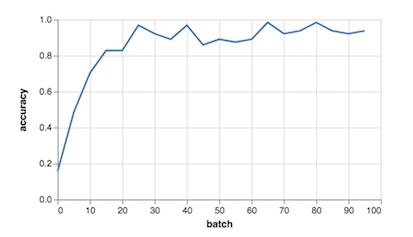
\includegraphics[keepaspectratio=true,width=\dimmin{}{\dimwidth{0.90}}]{images/tfjs}{}\mdline{222}%mdk
%mdk
\end{mdframe}\label{sec-using-a-convolutional-nn-to-recognize-hadwritten-digits}%mdk%mdk

%mdk-data-line={227}
\begin{mdframe}%mdk

\frametitle*{References}\label{heading-sec-references}%mdk%mdk

%mdk-data-line={229}
\noindent\mdline{229}https://en.wikipedia.org/wiki/Universal\mdline{229}\_\mdline{229}approximation\mdline{229}\_\mdline{229}theorem%mdk

%mdk-data-line={231}
\mdline{231}https://towardsdatascience.com/a-gentle-introduction-to-neural-networks-series-part-1-2b90b87795bc%mdk

%mdk-data-line={233}
\mdline{233}https://medium.com/all-of-us-are-belong-to-machines/the-gentlest-introduction-to-tensorflow-248dc871a224%mdk

%mdk-data-line={235}
\mdline{235}https://core.ac.uk/download/pdf/82123892.pdf%mdk

%mdk-data-line={237}
\mdline{237}http://www.cs.toronto.edu/\mdline{237}\textasciitilde{}\mdline{237}tijmen/csc321/lecture\mdline{237}\_\mdline{237}notes.shtml%mdk

%mdk-data-line={239}
\mdline{239}https://www.tensorflow.org/%mdk

%mdk-data-line={241}
\mdline{241}https://js.tensorflow.org/tutorials/%mdk
%mdk
\end{mdframe}\label{sec-references}%mdk%mdk%mdk%mdk%mdk


\end{document}
